\documentclass{article}

\usepackage{amssymb}
\usepackage[intlimits]{amsmath}
\usepackage{graphicx}
\usepackage{verbatim}
\usepackage{empheq}
\usepackage{bbm}
\usepackage{bm}
\usepackage{fullpage}
\usepackage{mathtools}
\usepackage{caption}
\usepackage{subcaption}
\usepackage{algorithm}
\usepackage{algpseudocode}
\usepackage{courier}

\usepackage{hyperref}
\hypersetup{
    colorlinks,
    citecolor=blue,
    filecolor=blue,
    linkcolor=blue,
    urlcolor=blue
}

\newcommand{\Prob}[1]{\ensuremath{\mathbb{P}\left[#1\right]}}
\newcommand{\CondP}[2]{\ensuremath{\mathbb{P}\left[#1|#2\right]}}
\newcommand{\Exp}[1]{\ensuremath{\mathbb{E}\left[#1\right]}}
\newcommand{\Var}[1]{\ensuremath{\text{Var}\left[#1\right]}}
\newcommand{\Std}[1]{\ensuremath{\text{Std}\left[#1\right]}}
\newcommand{\CondE}[2]{\ensuremath{\mathbb{E}\left[#1|#2\right]}}
\newcommand{\inner}[2]{\ensuremath{\left<#1,#2\right>}}
\newcommand*\widefbox[1]{\fbox{\hspace{2em}#1\hspace{2em}}}
\renewcommand{\(}{\left(}
\renewcommand{\)}{\right)}

\newcommand{\txtmathbf}[1]{\ensuremath{\text{\textbf{#1}}}}

\newtheorem{theorem}{Theorem}
\newtheorem{lemma}[theorem]{Lemma}
\newtheorem{claim}{Claim}
\newenvironment{proof}{{\bf Proof:}}{\hfill\rule{2mm}{2mm}}

\newtheorem{definition}{Definition}
\let\olddefinition\definition
\renewcommand{\definition}{\olddefinition\normalfont}

\DeclareMathOperator*{\argmin}{argmin}
\DeclareMathOperator*{\argmax}{argmax}

\graphicspath{{plots/}}

\title{CS155 Kaggle Project Report}
\author{Daniel Chao\thanks{Team partners listed alphabetically.} \and Jae Hong Kim\footnotemark[1]}
\date{\today} 

\begin{document}

\maketitle 
\tableofcontents 

\section{Overview}
The objective of the CS155 Kaggle project was to classify whether a financial report from a publically traded company was submitted to the U.S. Securities and Exchange Commission during the \href{http://en.wikipedia.org/wiki/Great_Recession}{Great Recession}.  

We are given data represented as a bag of words consisting of the most frequently occuring word stems. The training set consists of 4000 documents with their target labels while the testing set consists of 9868 documents. In addition to the bag of words representation, we are also given the tf-idf preprocessed version of the same dataset. Our approach to the project was to work exclusively with the tf-idf preprocessed data, which consisted of 500 features, and use ensemble selection \cite{caruana04} to pool over a large model library.  

Within our team, Jae focused on generating the model library using \texttt{scikit-learn}, and Daniel custom implemented ensemble selection using python according to the descriptions in R. Caruana's paper. Our code and implementations are in \href{https://github.com/jkim-/KaggleCS155}{this} github repository. 

Our team handle was ``DrOPitlikEitshot". 

\section{Generating the model library} \label{sec:models}
In this section, we present brief descriptions of the approximately 2000 models that make up our model library.  Each model consists of a unique combination of input processing and an instantiation of a learning algorithm that is used to transform and fit the training data set and predict the labels of the test data set.  All input processing and learning algorithms used were \texttt{scikit-learn} implementations.  

We note in particular that the model library is assembled without consulting the leader board. 

  \subsection{Input processing}

  \begin{itemize}
    \item \textbf{TF-IDF}: Term frequency-inverse document frequency, or tf-idf, is a feature representation of a collection of documents, or a corpus. By using a bag of words as the feature space, we can project a document in the corpus onto a numerical vector.  An example is a simple word count normalized by the total number of words, which suffers from inherent bias towards lesser meaningful words such as `the' and `is'.  Tf-idf attempts to overcome this by weighting the term frequency within a document by the overall term frequency across the entire corpus.  For this project, we are given both word count and tf-idf representations of the data.  Due to time constraints, we chose to make use of only the tf-idf data, which we deemed to be a more sensible representation for relative importance of keywords.

    \item \textbf{Centering and Scaling}: Centering is a transformation that subtracts the mean of the data set as to make the data have zero mean.  This removes any bias a feature might have from the way it was collected. Whereas centering is a uniquely defined procedure, scaling the data can be done in different ways. For our library, we employ two scaling methods, one is normalizing the data to unit variance (i.e. dividing each feature by its standard deviation) and the other is scaling each feature to be within a specified range (e.g. [-1, 1]).     

    \item \textbf{Feature Selection}: The training data set contains 4000 points, where each point is represented by a point in a 500-dimensional feature space.  We were concerned that the 500-demensional model would overfit the data, so we tried reducing the number of features using principal component analysis (PCA) and L1-based feature selection.

PCA can be used to rank a feature based on amount of information it carries, which is captured by its variance; the overall loss of information by reducing the feature space can be described by the reconstruction error $E_{\text{r}} = \|\mathbf{X}-\mathbf{X}_r\|^2$, or the Frobenius norm of difference between the originial design matrix and the reduced design matrix reconstructed in the originial feature space. Figure~\ref{fig:top-k} shows the reconstruction error as a function of the number of components kept for our training data set.  As we can see, the error decreases rapidly when the first few features are kept as they contain the most information.  For building the model library, we tried both keeping all features and reducing the number of features to 200, which corresponded to about $15\%$ reconstruction error.   

      \begin{figure}
	\centering
	  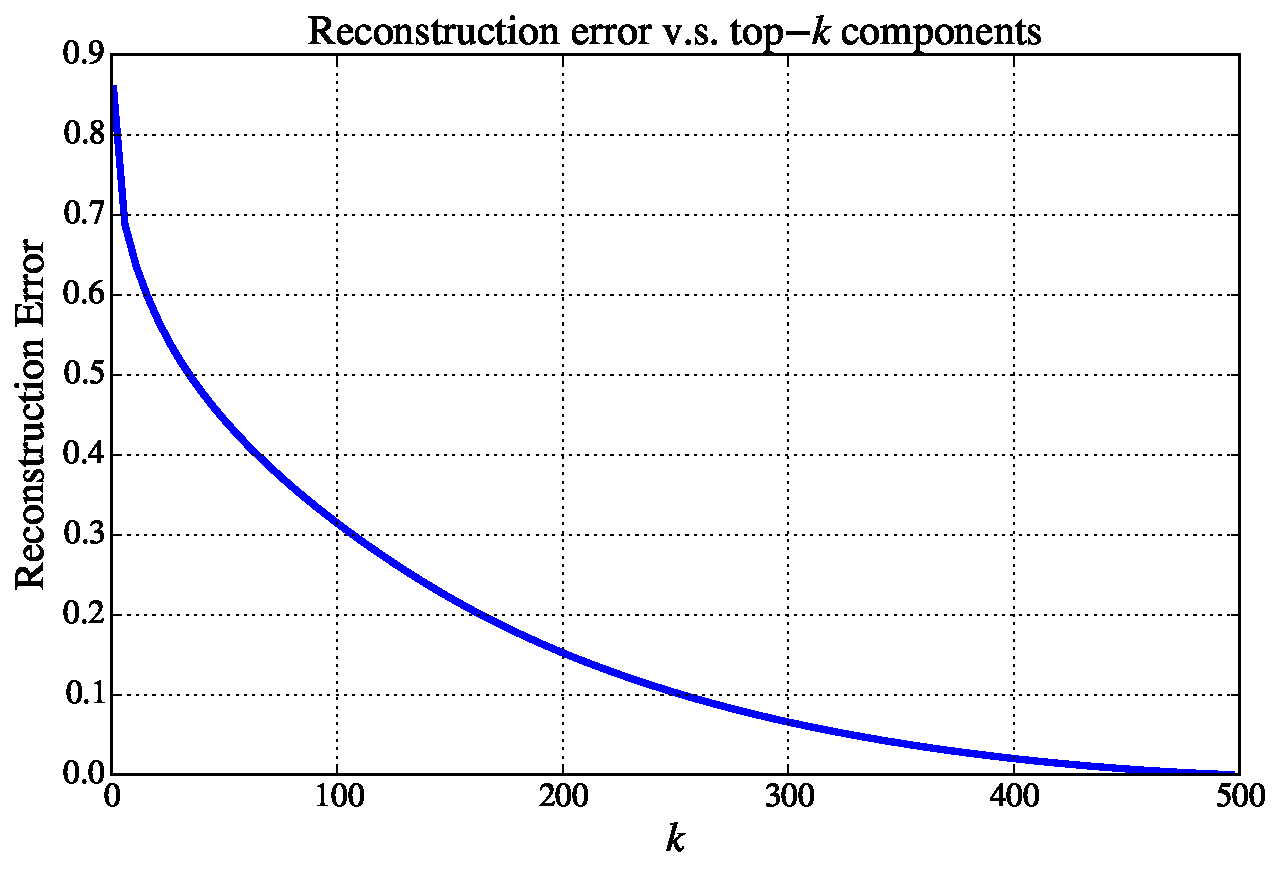
\includegraphics[width=0.4\textwidth]{top-k_PCA}
	\caption{}
	\label{fig:top-k}
      \end{figure}

L1-based feature selection uses the fact that linear models regularized by the L1-norm results in sparse solutions, resulting in another way to remove less important features.  The amount of reduction of feature space is control by the regularization parameter $C$ in the objective function.  For certain learners, we applied L1-based feature reduction using various values of $C:\{0.001, 0.01, 0.1\}$.

    \item \textbf{Whitening}: Whitening is a transformation that decorrelates a set of data.  Practically speaking, this is accomplish by transforming the covariance matrix of the data into an identity matrix (i.e. features are uncorrelated with unit variance).  It is clear that whitening, if done at all, should be done after feature selection.  As similar to feature selection, we explored the both options of learning on whitened and unwhitened data.   
  \end{itemize}
  
  \subsection{Learning algorithms}
  As most of the learning algorithms used in this project were discussed during class lectures, this section mostly aims to describe our approach to exploring the parameter space grid of each learner, where the reasonable starting values for the parameters were taken from the work by Niculescu-Mizil et al. \cite{KDD}.

  \begin{itemize}
    \item \textbf{Logistic Regression}: Logistic regression is a linear classification model that seeks to maximize the likelihood, or equivalently minimize the log loss.  In addition, the model can be regularized using either L1 or L2 penalty.  More concretely, logistic regression can be represented as the following optimization problem:
      \begin{equation} \label{eq:logreg}
	\argmin_{\mathbf{w}} \frac{1}{2}\|\mathbf{w}\|^2 + C\sum_i\log\left(\exp\left(-y_i\mathbf{x}_i^T\mathbf{w}\right)+1\right),
      \end{equation}
      where $\mathbf{x}_i$ and $y_i$ are the \emph{i}-th data point and its label, $\mathbf{w}$ is the vector of weights, and $C$ is the regularization parameter for the L1- or L2-norm of the weights.

      We generated the models for the library by first centering and normalizing the data, then varying the number of features used $\{200, 500\}$, the type of penalty used, $C:\{10^{-5}, 10^{-4}, 10^{-3}, 10^{-2}, \allowbreak 10^{-1}, 1, 10^{1}, 10^{2}\}$, whether to include a constant bias term in the log loss, and whether to balance the data to account for the fact that the training data consisted of $17\%$ of data with label $1$.  The data balancing was done either automatically based on the frequency of class labels or manually by weighting the label class $0/1$ by $1/3$, respectively. 

    \item \textbf{Support Vector Machine}: Support vector machine is a max-margin classifier, where the model tries to linearly separate the data while maximizing the distance between the separating hyperplane and the closest data points, which is the margin. In most cases, the data is not linearly separable due to noise, thus classifiers called soft-margin SVM's allow violation of the margin.  One forumation of soft-margin SVM is:
      \begin{equation} \label{eq:svm}
	\begin{split}
	  &\argmin_{\mathbf{w}} \frac{1}{2}\|\mathbf{w}\|^2 + C\sum_i\xi_i \\
	  &\text{subject to } y_i \left(\mathbf{w}^T \phi(\mathbf{x}_i)+b\right)\ge 1-\xi_i \text{ and } \xi_i \ge 0\;\forall i,
	\end{split}
      \end{equation}
      where $\xi_i$ is the the parameter representing the amount of violation allowed for \emph{i}-th data point and $\phi^T\phi$ is the kernel function which transforms the data into a higher dimensional represenation. 

      We generated many SVM models by first preprocessing the data to be scaled within the range [-1, 1] and then either reducing feature dimensions to 200 and whitening or not reducing and whitening.  The kernel functions used are: radial basis functions (RBF) for which we vary its width parameter $\gamma:\{0.001, 0.005, 0.01, 0.05, 0.1, 0.5, 1., 2.\}$, polynomials functions of degrees 2, 3, and 5, and a linear function. For all kernels, we vary the regularization parameter $C$ from $10^{-7}$ to $1000$ in factors of $10$.    

      After scoring the first set of models using cross validation, which will be described in Section~\ref{sec:ensemble} , we trained more SVM with RBF kernel with finer grid of $\gamma$ and $C$, and also balancing the data.

    \item \textbf{Boosted Decision Trees}: Boosting refers to iteratively learning a data set using a collection of "weak" learners, where a weak learner is a learned model with low predictive power.  This method takes adventage of the low variance of weak learners, while the inherently high bias of the weak learners are reduced by the ensemble nature of boosting.  The algorithm used for boosting this set of decision trees for classification is AdaBoost, and we vary the depth of the base classifier $\{1, 2, 3, 4, 5, 7, 10, 20\}$, number of rounds of boosting among 30 numbers between 1 and 1200, and the learning rate $\{0.7, 1\}$.  The learning rate acts as a regularizor for the model and may result in for better generalization.  The criterion used for splitting for the base classifier is the gini criterion. 

      We processed the inputs using centering and normalization, and then for some models reducing the feature space using L1-based feature selection using $C:\{10^{-3}, 10^{-2}, 10^{-1}\}$, where smaller value of $C$ implies larger reduction. Lastly, we also try balancing the data for some models.

    \item \textbf{Gradient Tree Boosting}: Gradient tree boosting is another method of boosting trees similar to AdaBoost.  Whereas AdaBoost is used only for classification, gradient boosting can be used for both regression and classification.  Although the concepts are similar, the differences in the algorithm might result is different generalization, thus we decided to include some models traine using gradient tree boosting.

      We generate different models by varying the number of rounds of boosting, the maximum depth of the base tree classifier, and the learning rate in a similar way as we did for the boosted decision trees. 

    \item \textbf{Random Forest}: In constrast to the boosting methods, random forest seeks to take adventage of the low bias and high predictive power of deeper and more complex decision trees.  As complex trees are prone to overfitting, random forest creates an ensemble of such trees where each tree is trained using different subsets of the data (bagging) and features. Bagging, or bootstrap aggregation, reduces the variance of the base classifiers and is not limited only to decision trees.    

      We generated various instantiations of random forest by varying the input processing, from centering and normalizing to feature selection using Lasso.  We tried learning on the raw unprocessed data, but the performance of those random forests were mediocre at best.  In addition, we vary the number of trees in the forest $\{256, 512, 1024\}$, the number of features to be considered for each split between 1 and 500, and the criterion for splitting between gini and information gain.  We also try balancing the data for some models.   
  \end{itemize}

\section{Ensemble selection} \label{sec:ensemble}
We first describe our implementation of ensemble selection, then we describe how it was used in our submission strategy.

\subsection{Ensemble selection implementation}
We wrote a custom python package that implements ensemble selection described in \cite{caruana04} and \cite{caruana06}. It is written specifically to work with \texttt{scikit-learn}; thus, many of our design decisions were based on the structure of its API. The key features that we implemented are listed below.
\begin{itemize}
  \item Forward stepwise selection: This is the main routine of ensemble selection and is described in the introduction of \cite{caruana04}. Notable features we implement are sorted ensemble initialization and model selection with replacement. All of these are described in detail in \cite{caruana04}. An additional feature we implement is early stopping in order to save CPU cycles for when the hill climbing error plateaus. 

  \item Ensemble bagging: This is way of to counter overfitting. It randomly chooses some prespecfied percentage of all available models and uses those as the model library for hill climbing. It then does this for some prespecified number of rounds and takes a vote among all bagged ensembles for the final decision. This procedure is described in detail in \cite{caruana04}.

  \item Cross-validated models: Since the efficacy of ensemble selection depends strongly on the size of the hill climbing set, we wanted to get the most out of the training data by using cross validation. We implemented the training and prediction of the so called ``cross-validated models'' described in \cite{caruana06}. This basically expands a single model to a team of $K$ models for $K$-fold cross validation. Predicting out of sample points is a vote among all $K$ team members, while predicting in sample points is the single decision of the member that did not train on the given point. 

  \item Model library pruning: We add an option to use just the top-$p$\% performing models in the base library. 
\end{itemize}

\subsection{Ensemble training and submission strategy}
Though our code was designed to be able to train any number of folds of cross validated models, we chose to uniformly train 5-fold models. In hindsight, this was too greedy as we did not anticipate the long time ensemble selection took to train and predict; probably a 2-fold strategy would have been more prudent given the time limit of the project. 

We specify a baseline ensemble model. These are based on the suggestions in \cite{caruana06}. The parameter settings are as follows:
\begin{itemize}
  \item Rounds of ensemble bagging: $20$.
  \item Percentage of models to use in each bag: $20\%$.
  \item Model pruning percentage: $20\%$. 
  \item Hill climbing early stopping: Fixed $15$ rounds of hillclimbing. This is suboptimal, but we had to truncate since we underestimated how long ensemble selection takes; however, the hillclimbing error did indeed plateau for most bag samples ($\approx 18$ out of $20$).
\end{itemize}
The ensemble training can be performed as the model library becomes ready. In practice, it is run whenever Jae reports that he has a bigger and better model library.

The way \cite{caruana04} views ensemble parameter tuning is as a type of regularization. In particular, tuning the bagging rounds, pruning percentage, etc. is akin to tuning $\lambda$ as in Lasso for example. We also take this view and use the leaderboard as the basis for tuning this ``$\lambda$''. In the end, we submit the following two ensembles assembled using the latest model library for final scoring:
\begin{enumerate}
  \item The baseline model: This is the model that is not influenced by how we are doing on the leaderboard. 
  \item The ensemble that does best on the leader board based on tuning the ensemble parameters: This is like tuning the regularization parameter on a held out sample. Unfortunately, we were not able to submit as many ensembles to Kaggle as we would have liked since certain parameter settings simply took too long to train or predict. 
\end{enumerate}


\section{Conclusion}
In the end, our performance was about average. 

The Achilles heel of our ensemble selection was that we were too greedy in choosing 5-fold vs smaller folds; e.g. 2-fold. Actually, we probably just underestimated how long ensemble selection would actually take; in our case, the running time was spent mostly on evaluating the individual \texttt{scikit-learn} models. Though many ensembles finished, we would have been able to better tune ensemble performance based on the leaderboard. 

For building the model library, it would have been better to explore a more diverse set of learning algorithms and models; e.g. neural network and unsupervised learning such as k-Nearest Neighbors. Another improvement would to also have a more systematic way of searching for well-performing regions in the parameter grid of each model. 

Furthermore, we didn't pursue taking advantage of existing structure in the data; e.g. sparsity and further feature extraction. 

\begin{thebibliography}{99}
\bibitem{caruana04}
  R. Caruana and A. Niculescu-Mizil.
  (2006).
  Ensemble selection from libraries of models.
  \emph{ICML '04}.
\bibitem{caruana06}
  R. Caruana, A. Munson, A. Niculescu-Mizil.
  (2006).
  Getting the Most Out of Ensemble Selection.
  \emph{Technical Report 2006-2045}.
\bibitem{KDD}
  A. Niculescu-Mizil \emph{et al}.
  (2009).
  Winning the KKD Cup Orange Challenge with Ensemble Selection.
  \emph{KDD Cup 2009}.

\end{thebibliography}

\end{document}
